%\documentclass{cumcmthesis}
\documentclass[withoutpreface,bwprint]{cumcmthesis} %去掉封面与编号页,电子版提交的时候使用。
\usepackage[final]{pdfpages}
\usepackage[linesnumbered,boxed,ruled,commentsnumbered]{algorithm2e}
\usepackage[framemethod=TikZ]{mdframed}
\usepackage{url}   % 网页链接
\usepackage{subcaption} % 子标题
\title{}
\tihao{A}
\baominghao{}
\schoolname{杭州电子科技大学}
\membera{ }
\memberb{ }
\memberc{ }
\supervisor{ }
\yearinput{2020}
\monthinput{08}
\dayinput{22}
\renewcommand\thesection{\arabic{section}.}

\begin{document}
	
	
	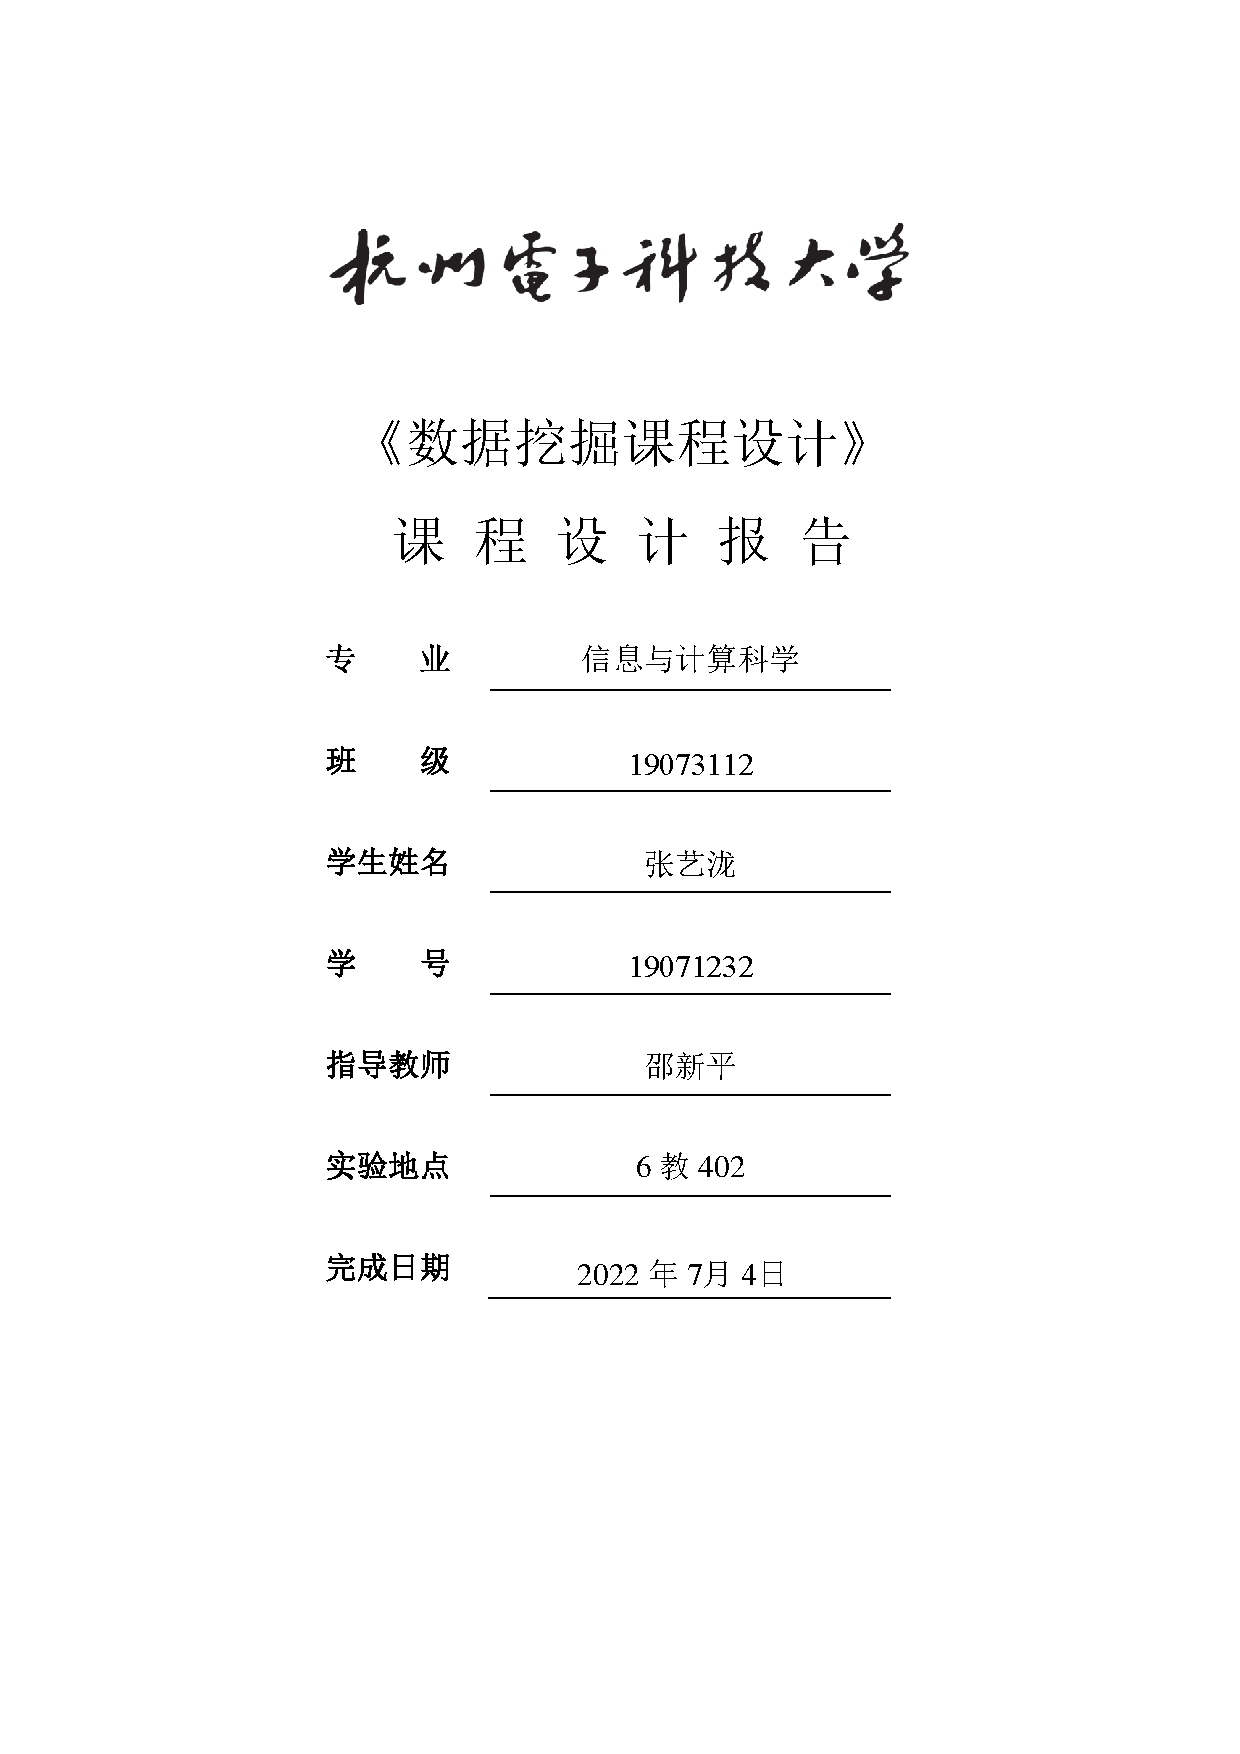
\includepdf{封面.pdf} 
	\newpage
	
	%目录
	\tableofcontents
	
	\newpage
	\section{背景}
	\subsection{数据挖掘背景}
	\par 1912年4月15日,在她的处女航中,被广泛认为是“永不沉没”的皇家邮轮泰坦尼克号在与冰山相撞后虽然生存中有一些运气因素,但似乎有些群体比其他群体更有可能生存下来。在本次挑战中,要求建立一个预测模型,以回答以下问题:“什么样的人更有可能存活?”使用乘客数据(即姓名、年龄、性别、社会经济阶层等)。
	
	\subsection{数据集介绍}
	\par 数据分为两组:训练集(train.csv)测试集(test.csv)
	训练集应用于构建机器学习模型。对于训练集,我们为每位乘客提供结果。您的模型将基于乘客性别和阶级等“特征”。您还可以使用特征工程来创建新特征。测试集应用于查看模型在未看到的数据上的性能。

	
\begin{figure}[H]
	\centering
	\centerline{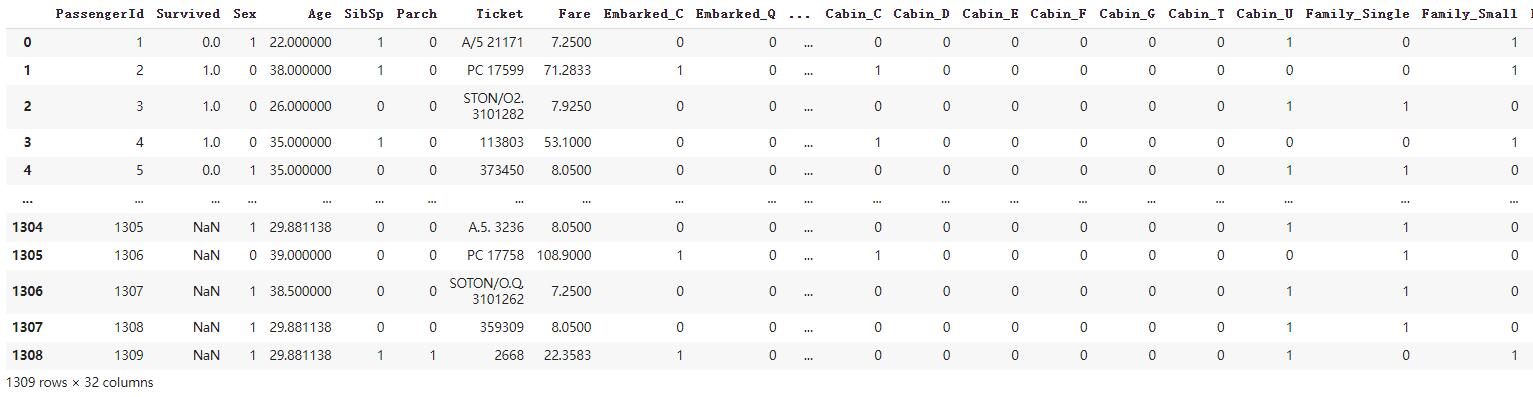
\includegraphics[width=\textwidth]{tai_2}}  
	\begin{center}
		\caption{数据集介绍}
	\end{center}
\end{figure}
	
	\section{数据预处理}
	\subsection{缺失值处理}
	\par 缺失值处理使用pd.fullna 函数,如果是数值类型,用平均值取代;如果是分类数据,用最常见的类别取代;使用模型预测缺失值,例如:K-NN。
	\par 对于年龄和船票价格,采用的是平均数来填充缺失值。对于登船港口,分别计算出各个类别的数量,采用最常见的类别进行填充。
	\par 对于船舱号,由于缺失的数据太多,将缺失的数据用’U’代替,表示未知。
	
	\subsection{数据分类}
	
	\par 数据分类的过程比较麻烦,对于有直接类别的数据还有字符串类型的数据进行了不同方式的处理。
	\par 乘客性别(Sex):男性 male,女性female	,令男性为1,女性为0
	\par 对于登船港口,客舱等级,客舱号,使用pd.get\_dummies进行独热编码,列名前缀是Embarked。
	
	\begin{figure}[H]
		\centering
		\centerline{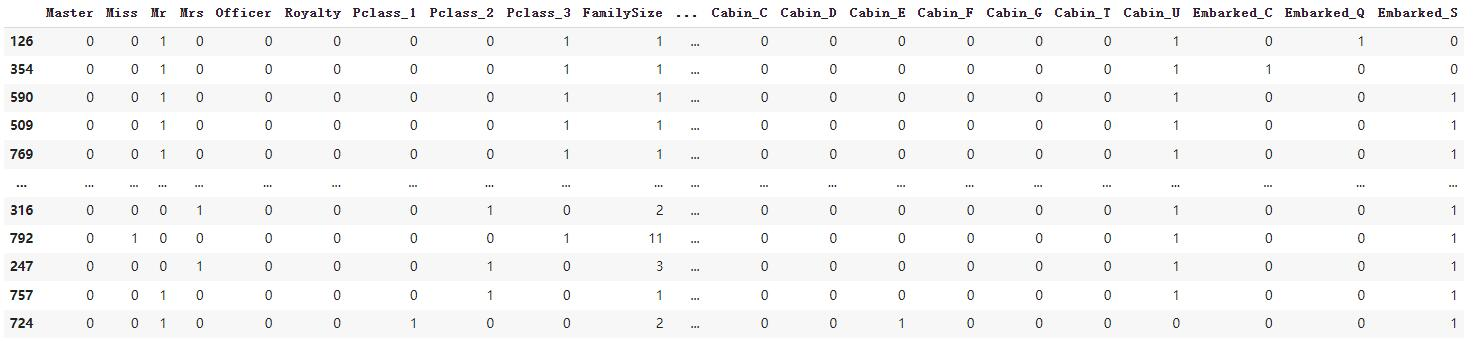
\includegraphics[width=\textwidth]{tai_1}}  
		\begin{center}
			\caption{数据预处理}
		\end{center}
	\end{figure}
	
\section{模型训练与评价}
\par 对于模型训练,使用sklearn库中的模型对数据进行训练。采用逻辑回归,随机森林,支持向量机,梯度提升决策,KNN,朴素贝叶斯分类多种算法进行训练并对其训练效果进行评价。
\subsection{逻辑回归}
\subsubsection{模型原理}
\par 二分类问题: 对样本点 x, 其标签$y \in\{0,1\} $,想要知道的是概率
\begin{align}
	\operatorname{Pr}(y=1 \mid x)
\end{align}
\par 对于二分类问题,显然可以建模假设  $y \mid x$  服从参数为  p  的Bernoulli分布,因此只需要估计 $ p=E(y \mid x) $

\par Bernoulli分布是二项分布  n=1  的特殊情形,显然也属于指数分布族。使用GLM建模:选择Bernoulli分布  +  正规连接,得到
\begin{align}
	p=\frac{1}{1+e^{-\beta^{T} x}}=s\left(\beta^{T} x\right)
\end{align}


\par 其中  $s(\cdot)$  称为 Sigmoid 函数
\begin{align}
s(z)=\frac{1}{1+e^{-z}}
\end{align}


\subsubsection{模型结果}
\par 经过运行,当训练集比测试集为8:2时,可以得到逻辑回归AUC=0.857。
\begin{lstlisting}
#逻辑回归
from sklearn.linear_model import LogisticRegression
model = LogisticRegression()
model.fit( train_X , train_y )
\end{lstlisting}

\begin{figure}[H]
	\centering
	\begin{minipage}[t]{0.48\textwidth}
		\centering
		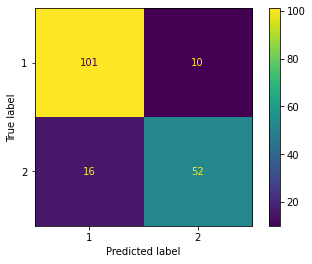
\includegraphics[width=6.3cm]{tai_R_1}
		\centerline{$\ \ \ \ \ \ \ \ \ \ $(a)}
	\end{minipage}
	\begin{minipage}[t]{0.48\textwidth}
		\centering
		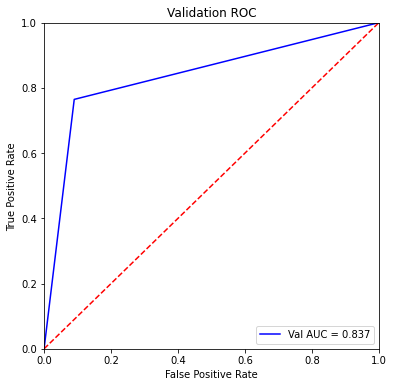
\includegraphics[width=6.3cm]{tai_R_2}
		\centerline{$\ \ \ \ \ \ \ \ \ \ $(b)}
	\end{minipage}
	
	\caption{结果可视化}
\end{figure}

\subsection{随机森林}
\subsubsection{模型原理}
\par  生成单棵决策树:
(1)训练总样本的个数为N,则单棵决策树从N个训练集中有放回的随机抽取n个作为此单颗树的训练样本。

(2)令训练样例的输入特征的个数为M,m远远小于M,则我们在每颗决策树的每个节点上进行分裂时,从M个输入特征里随机选择m个输入特征,然后从这m个输入特征里选择一个最好的进行分裂。m在构建决策树的过程中不会改变。这里注意,要为每个节点随机选出m个特征,然后选择最好的那个特征来分裂。

(3)每棵树都一直这样分裂下去,直到该节点的所有训练样例都属于同一类。不需要剪枝。由于之前的两个随机采样的过程保证了随机性,所以就算不剪枝,也不会出现over-fitting。


\subsubsection{模型结果}
\par 经过运行,当训练集比测试集为8:2时,可以得到逻辑回归AUC=0.837。
\begin{lstlisting}
#随机森林Random Forests Model
from sklearn.ensemble import RandomForestClassifier
model = RandomForestClassifier(n_estimators=100)
model.fit( train_X , train_y )

\end{lstlisting}

\begin{figure}[H]
	\centering
	\begin{minipage}[t]{0.48\textwidth}
		\centering
		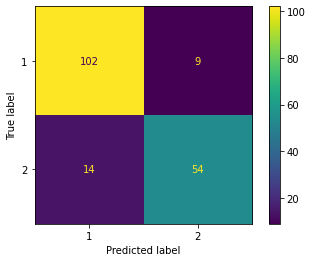
\includegraphics[width=6.3cm]{tai_l_1}
		\centerline{$\ \ \ \ \ \ \ \ \ \ $(a)}
	\end{minipage}
	\begin{minipage}[t]{0.48\textwidth}
		\centering
		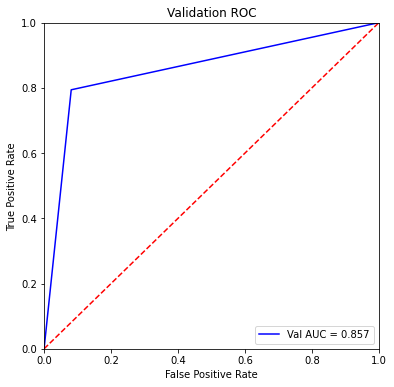
\includegraphics[width=6.3cm]{tai_l_2}
		\centerline{$\ \ \ \ \ \ \ \ \ \ $(b)}
	\end{minipage}
	
	\caption{结果可视化}
\end{figure}



\subsection{支持向量机}
\subsubsection{模型原理}
\par SVM是一种二类分类模型。它的基本模型是在特征空间中寻找间隔最大化的分离超平面的线性分类器。·当训练样本线性可分时,通过硬间隔最大化,学习一个线性分类器,即线性可分支持向量机;
·当训练数据近似线性可分时,引入松弛变量,通过软间隔最大化,学习一个线性分类器,即线性支持向量机;
·当训练数据线性不可分时,通过使用核技巧及软间隔最大化,学习非线性支持向量机。
硬间隔最大化(几何间隔)、学习的对偶问题、软间隔最大化(引入松弛变量)、非线性支持向量机(核技巧)。



\subsubsection{模型结果}
\par 经过运行,当训练集比测试集为8:2时,可以得到逻辑回归AUC=0.618。
\begin{lstlisting}
 #支持向量机Support Vector Machines
from sklearn.svm import SVC
model = SVC()
model.fit( train_X , train_y )
\end{lstlisting}

\begin{figure}[H]
	\centering
	\begin{minipage}[t]{0.48\textwidth}
		\centering
		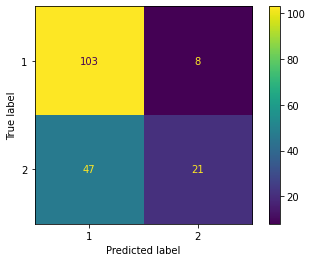
\includegraphics[width=6.3cm]{tai_S_1}
		\centerline{$\ \ \ \ \ \ \ \ \ \ $(a)}
	\end{minipage}
	\begin{minipage}[t]{0.48\textwidth}
		\centering
		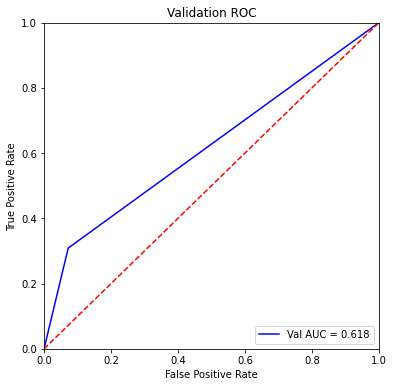
\includegraphics[width=6.3cm]{tai_S_2}
		\centerline{$\ \ \ \ \ \ \ \ \ \ $(b)}
	\end{minipage}
	
	\caption{结果可视化}
\end{figure}



\subsection{梯度提升决策}
\subsubsection{模型原理}
\par  GBDT是通过采用加法模型(即基函数的线性组合),以及不断减小训练过程产生的残差来达到将数据分类或者回归的算法, Friedman提出了利用最速下降的近似方法,利用利用损失函数的负梯度在当前模型的值,作为回归问题中提升树算法的残差的近似值,拟合一个回归树。
\begin{align}
-\left[\frac{\partial L\left(y_{i}, F\left(\mathbf{x}_{\mathbf{i}}\right)\right)}{\partial F\left(\mathbf{x}_{\mathbf{i}}\right)}\right]_{F(\mathbf{x})=F_{t-1}(\mathbf{x})}
\end{align}

\subsubsection{模型结果}
\par 经过运行,当训练集比测试集为8:2时,可以得到逻辑回归AUC=0.846。
\begin{lstlisting}
#梯度提升决策分类Gradient Boosting Classifier
from sklearn.ensemble import GradientBoostingClassifier
model = GradientBoostingClassifier()
model.fit( train_X , train_y )
\end{lstlisting}

\begin{figure}[H]
	\centering
	\begin{minipage}[t]{0.48\textwidth}
		\centering
		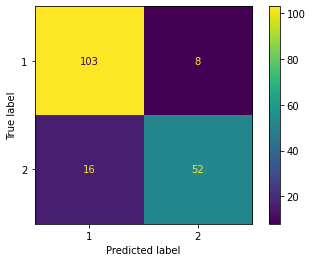
\includegraphics[width=6.3cm]{tai_G_1}
		\centerline{$\ \ \ \ \ \ \ \ \ \ $(a)}
	\end{minipage}
	\begin{minipage}[t]{0.48\textwidth}
		\centering
		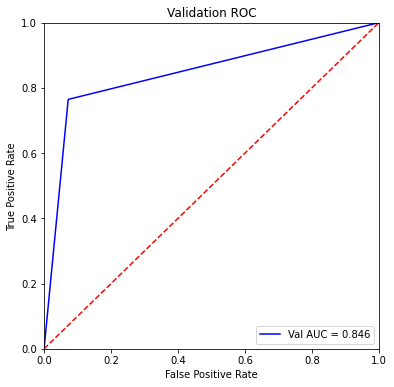
\includegraphics[width=6.3cm]{tai_G_2}
		\centerline{$\ \ \ \ \ \ \ \ \ \ $(b)}
	\end{minipage}
	
	\caption{结果可视化}
\end{figure}




\subsection{KNN}
\subsubsection{模型原理}
\par KNN分类算法包括以下4个步骤:
\begin{itemize}
\item 准备数据,对数据进行预处理  。
\item 计算测试样本点(也就是待分类点)到其他每个样本点的距离。
\item 对每个距离进行排序,然后选择出距离最小的K个点。
\item 对K个点所属的类别进行比较,根据少数服从多数的原则,将测试样本点归入在K个点中占比最高的那一类
\end{itemize}

\subsubsection{模型结果}
\par 经过运行,当训练集比测试集为8:2时,可以得到逻辑回归AUC=0.781。
\begin{lstlisting}
#KNN最邻近算法 K-nearest neighbors
from sklearn.neighbors import KNeighborsClassifier
model = KNeighborsClassifier(n_neighbors = 3)
model.fit( train_X , train_y )
\end{lstlisting}

\begin{figure}[H]
	\centering
	\begin{minipage}[t]{0.48\textwidth}
		\centering
		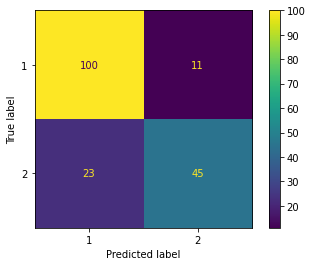
\includegraphics[width=6.3cm]{tai_K_1}
		\centerline{$\ \ \ \ \ \ \ \ \ \ $(a)}
	\end{minipage}
	\begin{minipage}[t]{0.48\textwidth}
		\centering
		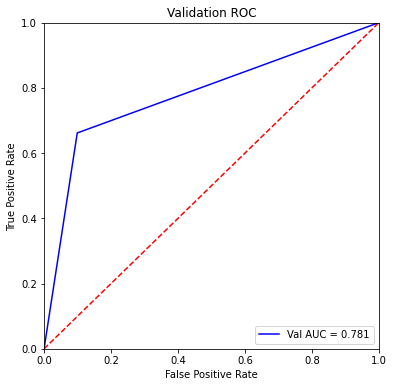
\includegraphics[width=6.3cm]{tai_K_2}
		\centerline{$\ \ \ \ \ \ \ \ \ \ $(b)}
	\end{minipage}
	
	\caption{结果可视化}
\end{figure}





\subsection{朴素贝叶斯分类}
\subsubsection{模型原理}
\par 朴素贝叶斯分类(NBC)是以贝叶斯定理为基础并且假设特征条件之间相互独立的方法,先通过已给定的训练集,以特征词之间独立作为前提假设,学习从输入到输出的联合概率分布,再基于学习到的模型,输入X求出使得后验概率最大的输出Y。

由于  $P(X)$  的大小是固定不变的,因此在比较后验概率时,只比较上式的分子部分即可。因此可以得到一个样本数据属于类 别 $ y_{i} $ 的朴素贝叶斯计算:


\begin{align}
P\left(y_{i} \mid x_{1}, x_{2}, \cdots, x_{d}\right)=\frac{P\left(y_{i}\right) \prod_{j=1}^{d} P\left(x_{j} \mid y_{i}\right)}{\prod_{j=1}^{d} P\left(x_{j}\right)}
\end{align}
\subsubsection{模型结果}
\par 经过运行,当训练集比测试集为8:2时,可以得到逻辑回归AUC=0.819。
\begin{lstlisting}
#朴素贝叶斯分类 Gaussian Naive Bayes
from sklearn.naive_bayes import GaussianNB
model = GaussianNB()
model.fit( train_X , train_y )
\end{lstlisting}

\begin{figure}[H]
	\centering
	\begin{minipage}[t]{0.48\textwidth}
		\centering
		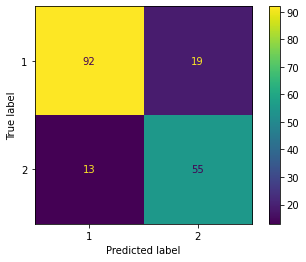
\includegraphics[width=6.3cm]{tai_B_1}
		\centerline{$\ \ \ \ \ \ \ \ \ \ $(a)}
	\end{minipage}
	\begin{minipage}[t]{0.48\textwidth}
		\centering
		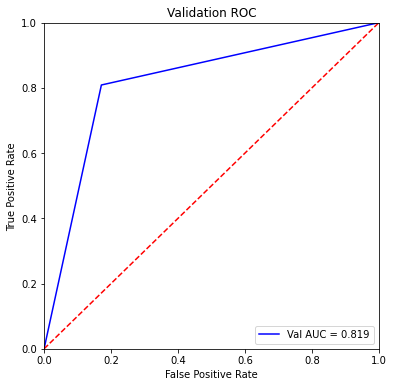
\includegraphics[width=6.3cm]{tai_B_2}
		\centerline{$\ \ \ \ \ \ \ \ \ \ $(b)}
	\end{minipage}
	
	\caption{结果可视化}
\end{figure}




\subsection{模型评价}
\par 设置训练集数据与测试集数据范围为0.6-0.9,计算各个模型的分数,可以得到下图:

	\begin{figure}[H]
	\centering
	\centerline{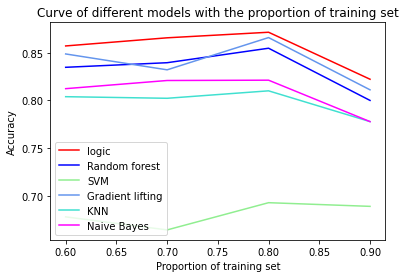
\includegraphics[width=0.9\textwidth]{tai_p_1}}  
	\begin{center}
		\caption{数据预处理}
	\end{center}
\end{figure}
\par 可以看到,效果最好的为逻辑回归模型。



	
\end{document} 